\documentclass{upmassignment}
\usepackage[spanish]{babel}
\usepackage{ifthen}
\usepackage{amsmath}
\usepackage{amsfonts}

%% PGFPLOTS %%
\usepackage{pgfplots}

%% TIKZ %%
\usepackage{tikz}
\usetikzlibrary{babel}
\usepackage{animate}
\usetikzlibrary{positioning}
\usetikzlibrary{shapes,arrows, positioning, calc}
\usetikzlibrary{overlay-beamer-styles}
\usetikzlibrary{chains,shapes.multipart}
\usetikzlibrary{scopes}
\usetikzlibrary{automata}
\usetikzlibrary{positioning}  %                 ...positioning nodes
\usetikzlibrary{arrows}       %                 ...customizing arrows
\usetikzlibrary{intersections}


% Para mostrar/ocultar soluciones
\newboolean{show}
%\setboolean{show}{true}
\setboolean{show}{false}
\usepackage{environ}
\NewEnviron{solucion}{
  \ifshow
      \begin{answer}\BODY\end{answer}
  \fi}


%% MATH commands
\DeclareMathOperator{\Var}{Var}




\coursetitle{Creating assignments}
\courselabel{RSTC}
\exercisesheet{Ejercicio de Alumno}{Temas 6 y 7}
\student{\ }%
\semester{Segundo Semestre}
\date{\today}
\university{Universidad Politécnica de Madrid}
\school{Departamento de Ingeniería de Sistemas Telemáticos}
%\usepackage[pdftex]{graphicx}
%\usepackage{subfigure}


\setlength{\textwidth}{5.0in}
\linespread{1.3}
\renewcommand{\PB}{{\bfseries Problema}}















\begin{document}

Se pretende modelar qué va a suceder en
el próximo Gran Premio de F1 de
Emilia-Romagna --
\textit{Autodromo Enzo e Dino Ferrari}.

\vspace{1em}

\begin{minipage}{\textwidth}
    \centering
    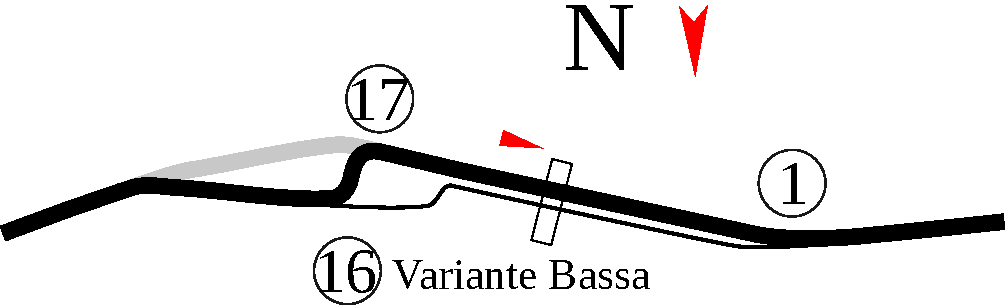
\includegraphics[width=.4\textwidth]{figs/box-pitlane.pdf}
\end{minipage}

\begin{problemlist}
    \pbitem El acceso a boxes tiene
    200 [m], un carril
    límite de velocidad de
    80 [km/h], y el tiempo de llegada
    entre coches es exponencial de media
    5~[sec]. ¿Cuál será entonces el tiempo
    medio de acceso a boxes?

    \begin{solucion}
        \input{../../RSTC-solutions/tema-7/solucion-problema-1.tex}
    \end{solucion}


    \pbitem Verstappen (VER)
    y Pérez (PER) se han parado en pista.

    \vspace{1em}
    \begin{tikzpicture}[scale=0.6, every node/.style={scale=0.6}]
        \draw (0,0) -- (10,0);
        \draw (0,2) -- (10,2);
        \draw[dashed] (0,1) --
            (6.7,1);
        \draw[dashed] (7.3,1) -- (10,1);

        % RB cars
        \node[rectangle,draw,rotate=20] at
            (2,1.5) {PER};
        \node[rectangle,draw,rotate=70] at
            (7,1.2) {VER};

        \draw [->,thick] (0.2,1.5) to[out=-45,in=180] (2,.5) to[out=0,in=180] (10.5,0.2)
            node[rectangle,draw,
            anchor=west]
            {ALO};

    \end{tikzpicture}
    \vspace{1em}

    El resto de pilotos 
    tardan, en media, un tiempo exponencial de
    0.5~[sec] en cruzar a PER, y 1~[sec] en
    cruzar a VER. Como el
    tiempo entre pilotos es una
    exponencial de media 2~[sec], ¿cuánto
    tiempo tardan, en media, en pasar a
    PER y VER?

    \begin{solucion}
        \input{../../RSTC-solutions/tema-7/solucion-problema-2.tex}
    \end{solucion}


    \pbitem El team radio de F1
    usa $N$ canales en frecuencia para
    transmitir mensajes de 20 pilotos.
    Cada canal tarda un tiempo exponencial
    en transmitir los mensajes, y tiene
    una tasa de 100~[paquetes/sec].
    Los pilotos reciben un flujo de voz de
    10~[paquetes/sec], y si los canales 
    están ocupados, el mensaje espera en cola.
    ¿Cuántos canales radio debe haber para
    que la probabilidad de espera de un
    mensaje sea menor del 10\%?

    \begin{minipage}{\textwidth}
        \centering
        \resizebox{!}{.27\textwidth}{%
            \begin{tikzpicture}[
declare function={free(\k,\I)=\I^\k/(\k!);}
]




%%%% DEFINE SUMATION USING
%https://tex.stackexchange.com/a/526600/62559
\newcounter{isum}
\pgfplotsset{summand/.initial=max}
\pgfmathdeclarefunction{sum}{2}{%
\begingroup%
\pgfkeys{/pgf/fpu,/pgf/fpu/output format=fixed}%
\edef\myfun{\pgfkeysvalueof{/pgfplots/summand}}%
\pgfmathsetmacro{\mysum}{0}%
\pgfmathsetmacro{\myx}{#2}%
\pgfmathtruncatemacro{\imax}{#1}%
\setcounter{isum}{0}%
\loop
\pgfmathsetmacro{\mysum}{\mysum+\myfun(\value{isum},#2)}%
\ifnum\value{isum}<\imax\relax
\stepcounter{isum}\repeat
\pgfmathparse{\mysum}%
\pgfmathsmuggle\pgfmathresult\endgroup%
}%







\begin{axis}[every axis plot post/.append style={
  mark=none,samples=100},
  axis x line*=bottom,
  axis y line*=left,
  xlabel={$A$},
  ylabel={$E_C(N,A)$},
  ymode=log,
  ymin=10e-4,
  ymax=1,
  enlargelimits=upper,
  grid=both,
  width=4in,
  height=2in]

  % N=3
  \pgfmathsetmacro{\N}{3}
  \addplot+[summand=free,ultra thick, smooth,
          color=HotPink1,domain=0:3] {
      \x^\N/\N! * 1/(1-\x/\N)
      *1/( sum(\N-1,\x)+x^\N/\N!* 1/(1-\x/\N) )}
      node [midway,anchor=south west] {};

  % N=4
  \pgfmathsetmacro{\N}{4}
  \addplot+[dashed,summand=free,ultra thick, smooth,
          color=HotPink2,domain=0:4] {
      \x^\N/\N! * 1/(1-\x/\N)
      *1/( sum(\N-1,\x)+x^\N/\N!* 1/(1-\x/\N) )}
      node [pos=0.3,anchor=west] {};


  % N=5
  \pgfmathsetmacro{\N}{5}
  \addplot+[summand=free,ultra thick, smooth,
          color=HotPink3,domain=0:5] {
      \x^\N/\N! * 1/(1-\x/\N)
      *1/( sum(\N-1,\x)+x^\N/\N!* 1/(1-\x/\N) )}
      node [pos=.5,anchor=east] {};

  % N=6
  \pgfmathsetmacro{\N}{6}
  \addplot+[dashed,summand=free,ultra thick, smooth,
          color=HotPink4,domain=0:5] {
      \x^\N/\N! * 1/(1-\x/\N)
      *1/( sum(\N-1,\x)+x^\N/\N!* 1/(1-\x/\N) )}
      node [pos=.5,anchor=east] {};

  \legend{$N=3$,$N=4$,$N=5$,$N=6$}









\end{axis}



\end{tikzpicture}


        }
    \end{minipage}

    \begin{solucion}
        \input{../../RSTC-solutions/tema-7/solucion-problema-3.tex}
    \end{solucion}
\end{problemlist}

\end{document}


